\documentclass{article}

\usepackage{graphicx}
\usepackage[utf8]{inputenc}
\usepackage[T1]{fontenc}

\newcommand{\id}[1]{\mbox{\textit{#1}}}


\title{Large-scale Information Extraction from Neuroscientific Literature}
\date{Spring 2015}
\author{Marco Antognini}

\begin{document}

\maketitle

Master Semester Project under the supervision of:
Jean-Cédric Chappelier \& 
Renaud Richardet
Artificial Intelligence Laboratory LIA - EPFL

\pagenumbering{gobble}
\newpage
\pagenumbering{arabic}


\tableofcontents
\newpage


\section{Introduction}

TODO describe bluima and sherlok and the context.


\section{Packaging}

One of the first objective of this project was the disassociation of algorithms (engine annotators) and their different resources (model files) and devise a packaging system, based on Maven, that would be flexible while being simple and convenient to use and let the user define pipelines using specific annotators and models.

The main idea is to store a set of resources, such as dataset trained on a specific corpus of texts, in a jar file and access them in read-only mode at runtime. Package dependencies can be used to ensure that some files are available at runtime and ideally package version should be used to let the user update resources independently of the algorithms.

Here we describe three alternatives -- namely A, B and C -- that we considered before deciding on a fourth variant. Below, \id{ada} and \id{bob} denote two variants of a kind of resource that are compatible with a common algorithm package, denoted \id{algo}. The \id{using*} packages can be thought as pipelines in the context of bluima/sherlok.

\subsection{Version A}

The first system we analysed spread each algorithm and set of resources into an individual package that depends on \id{modeldep}, a proxy utility to access the resource files inside jar archives. If an algorithm depends on some resource file then it accepts as input parameter the model name (as a string) and use the proxy to load the file. In this scenario pipeline packages have dependencies toward their annotators but also toward specific models as shown in figure \ref{fig:pkgsysA}.

This system has several positive aspects. First of all, tests can be easily written by specifying potentially multiple resource packages as dependencies with Maven's test scope. Then, \id{modeldep} also defines a clear Java interface to define the contract for models and their versions. Additionally, the proxy system centralises in only one place the utility to load resources and therefore ease maintenance by not involving code duplication in several packages. However, models could not be swapped on the fly since it would involve recompiling and repackaging \id{using\_my\_algo}.  Alternatively, to prevent being modified, \id{using\_my\_algo} could depend on both \id{ada} and \id{bob} packages but this would not be as flexible as we want it to be.

\begin{figure}
\centering
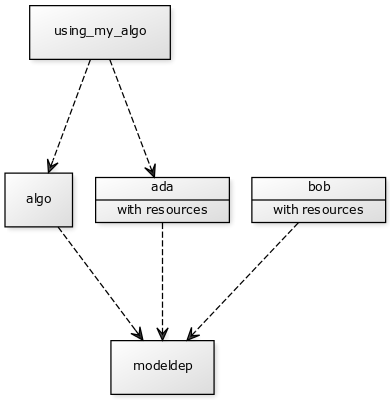
\includegraphics{res/packaging_version_A.png}
\caption{Packaging Version A}
\label{fig:pkgsysA}
\end{figure}


\subsection{Version B}

The second approach is based on Maven's version string: an \id{algo} will depend on an abstract \id{model} which provide a mechanism to load a specific file from its jar archive and both \id{ada} and \id{bob} model versions are defined as subversion of \id{model}. For example, if \id{model} is defined as version \id{0.1} then \id{ada} will use the string \id{0.1-ADA} to define its version and the \id{algo} will accept versions in the range $ [0.1,0.2) $.

The model actually used will be either specified at compile time (cf. \id{using.algo2}) or be selected at runtime depending on the installed packages (cf. \id{using.algo1}) as depicted on Figure \ref{fig:pkgsysB}. While this offers a great flexibility to the user designing pipelines and allows him to swap models without repackaging anything, it means that test projects cannot ensure the correctness of more than one model version at a time. Moreover, if no specific version is bound to the pipeline, such as with \id{using.algo1}, then there is no strong guarantee that a valid version is available at runtime.

\begin{figure}
\centering
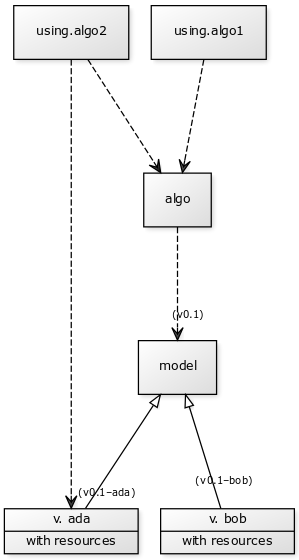
\includegraphics{res/packaging_version_B.png}
\caption{Packaging Version B}
\label{fig:pkgsysB}
\end{figure}


\subsection{Version C}

The third version we studied is the most simple one: as illustrated on Figure \ref{fig:pkgsysC}, instead of splitting everything in separate package, only annotators are packaged independently of pipelines and resources, which are grouped together. On the one hand this system couldn't be simpler but on the other, since pipelines often involve several engine annotators that are themselves used in several pipelines, the coupling of models and the corresponding algorithm implies that many packages have to be created to support each combination of models.


\begin{figure}
\centering
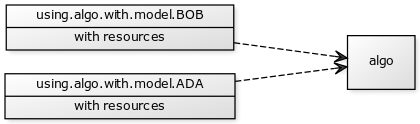
\includegraphics{res/packaging_version_C.png}
\caption{Packaging Version C}
\label{fig:pkgsysC}
\end{figure}


\subsection{Conclusion}

After exploring possibilities offered by the Maven packaging system we analysed how resources and engines are related to each others and used by pipelines in bluima. Figure \ref{fig:pkgsysD} depicts those relations. It was also considered that repackaging is an acceptable cost to swap models. The most important point was avoiding at all cost to package an exponentially huge number of pipelines to match each and every possible combinations and for this reason version C was discarded.

We also reflected on the structure of the algorithm, especially on their input arguments. We came to the conclusion that, mostly for flexibility, they should accept \id{InputStream}s as input and not be bound to any models. Instead, the pipelines will be in charge to give them the proper resource data streams. Therefore the pipeline will have dependencies toward algorithms and models.

Finally, in order to centralise code and simplify loading resources we introduce \id{ModelProxy}, a utility class used by pipelines that, given a string representing class name, open a stream to a given file inside the class' jar archive.

\begin{figure}
\centering
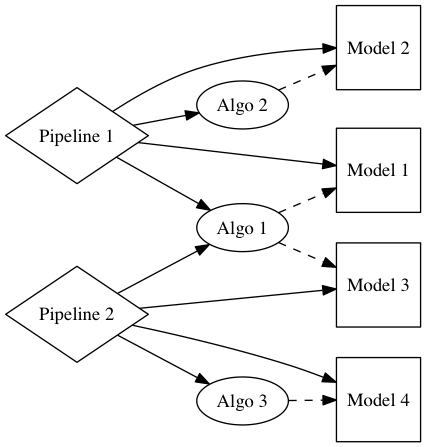
\includegraphics{res/packaging_version_D.png}
\caption{Packaging Version D}
\label{fig:pkgsysD}
\end{figure}

%\newpage
%\begin{appendix}
%  \listoffigures
%  \listoftables
%\end{appendix}

\end{document}
